\section{cmc 决赛备考}

\begin{enumerate}
	\item \textbf{优先采用教材上提供的基本方法和自然的思路.}
	\item \textbf{换序问题在时间比较富裕的情况下一定要严格证明.}
	\item \textbf{中值定理一定是自然的构造, 不要想的奇奇怪怪.}
	\item \textbf{填空题是基本盘, 一定不能错, 多检查, 可以猜答案.}
	\item \textbf{遇事不绝, 分部积分.}
	\item \textbf{遇事不绝, 不妨设标准型.}
	\item \textbf{数学类高年级组误判率较高! \underline{重代数轻分析}!}
	\item \textbf{第一天考完下午和晚上是最好玩的, 抓紧时机面基各路大神, 笔者当初考完带着一堆小伙伴去撸串, 干了十瓶可乐.}
	\item \textbf{考完当天晚上就会出成绩, 误判几率不低, 可以尽力配合老师查分.}
\end{enumerate}

\section{线性代数}

\begin{itemize}
	\item Jordan 分解
	\item 同时(正交)相似上三角/对角化\footnote{正交性要求特征值全为实数,或者实对称...}
	\item 两个半正定矩阵 $A,B$ 可以同时合同对角化.
	\item 实对称矩阵和正定矩阵显然可以同时合同对角化
	\item 矩阵打洞
	\item 摄动法,可以不妨设可逆
	\item $AB$ 和 $BA$ 有完全一样的非零 Jordan 块
	\item 与所有可逆矩阵可交换的矩阵是数量矩阵 $\lambda I$.
	\item 对 $A\in \mathbb{R}^{m\times n}$,有 $r(A^{T}A)=r(A)$.
	\item $r(A)=\dim \mathrm{Im}A=n-\dim \ker A$.
	\item $A$ 是半正定矩阵,等价于 $A$ 所有主子式\footnote{主子式是指取任意行和对应的列交叉出来的子式的行列式,代数主子式还要考虑逆序数.}非负,等价于 $A$ 的所有特征值为非负实数,等价于存在 $C\in \mathbb{R}^{n\times n}$ 使得 $A=C^{T}C$.
	\item 若 $A$ 可逆,则 $A^{-1}$ 是 $A$ 的多项式. 考虑特征多项式和哈密顿凯莱定理 (结合 $a_0\neq0$)
	\item $A^{*}$ 是 $A$ 的多项式. 注意到 $A^{*}=\lvert A \rvert A^{-1}$.
	\item 瑞丽商
	\item 反对称实矩阵的特征值实部为 0.
	\item 循环行列式
	\item 求解 $AX-XB=C$. 有唯一解的充要条件是 $A,B$ 无相同特征值. 证明考虑分块 Jordan 爆算. 这也是对于 $AX=XB$ 交结数的证明.
	\item 特征多项式等于极小多项式的等价条件.
	\item 覆盖定理
	\item 实正规矩阵\footnote{$AA^{T}=A^{T}A$}的正交相似标准型.
	\item 相似的正规矩阵必然酉相似. 若为实正规,则正交相似.
	\item 酉相似\underline{实}矩阵必然实正交相似.
	\item $A$ 是复正规矩阵的充要条件是 $A$ 的共轭转置是 $A$ 的多项式
	\item 三对角矩阵的行列式递推
	\item Perron 判别法
\end{itemize}

\begin{figure}[H]
\centering
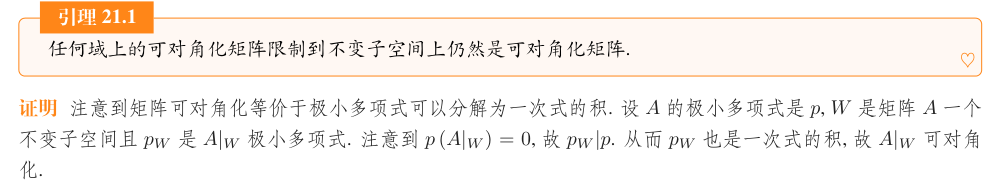
\includegraphics[width=\textwidth]{cmc决赛-2025040617.png}
% \caption{}
\label{}
\end{figure}
\begin{figure}[H]
\centering
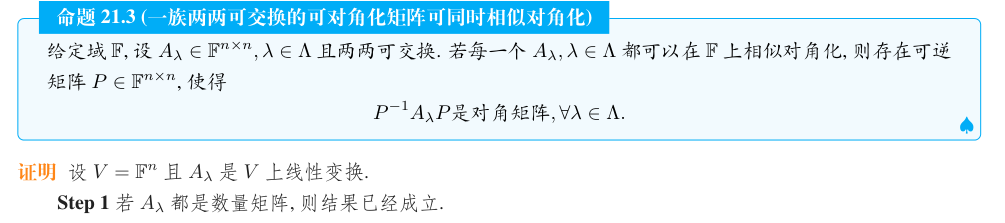
\includegraphics[width=\textwidth]{1-cmc决赛-2025040617.png}
% \caption{}
\label{}
\end{figure}
\begin{figure}[H]
\centering
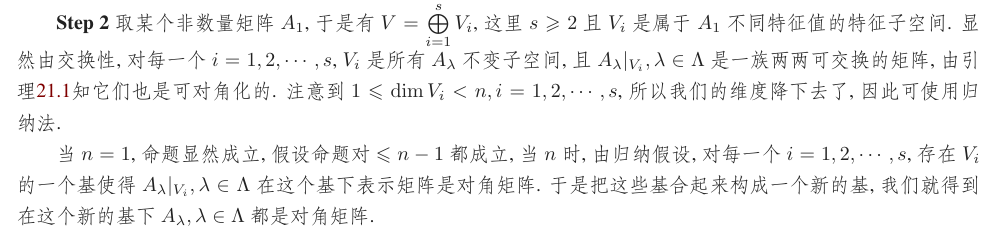
\includegraphics[width=\textwidth]{2-cmc决赛-2025040617.png}
% \caption{}
\label{}
\end{figure}
\begin{figure}[H]
\centering
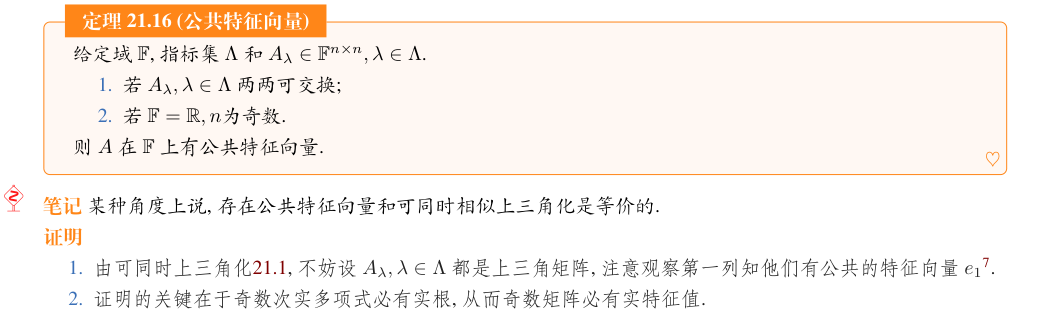
\includegraphics[width=\textwidth]{3-cmc决赛-2025040617.png}
% \caption{}
\label{}
\end{figure}
\begin{figure}[H]
\centering
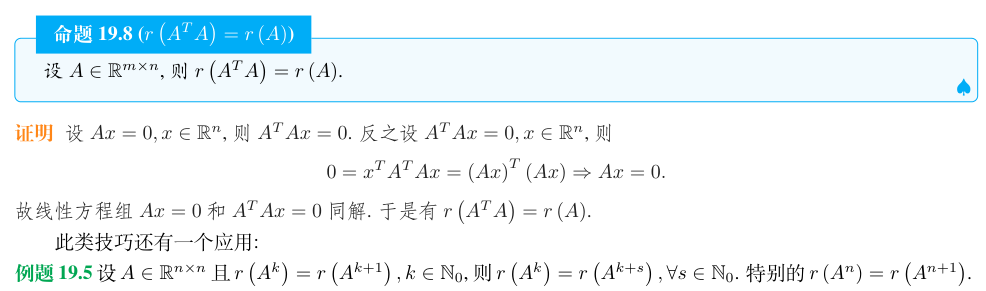
\includegraphics[width=\textwidth]{3-cmc决赛-2025040618.png}
% \caption{}
\label{}
\end{figure}
\begin{figure}[H]
\centering
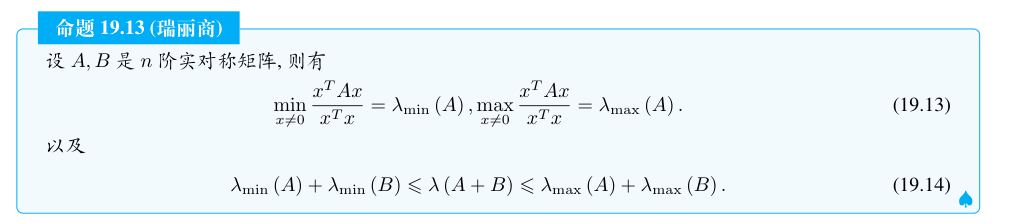
\includegraphics[width=\textwidth]{4-cmc决赛-2025040618.png}
% \caption{}
\label{}
\end{figure}
\begin{figure}[H]
\centering
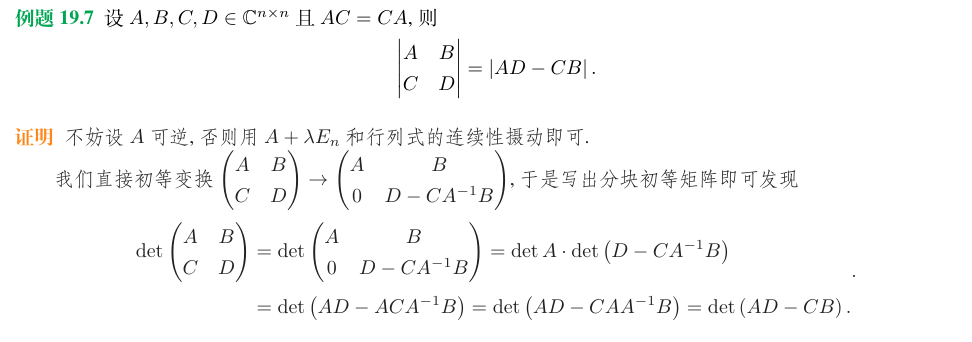
\includegraphics[width=\textwidth]{5-cmc决赛-2025040618.png}
% \caption{}
\label{}
\end{figure}
\begin{figure}[H]
\centering
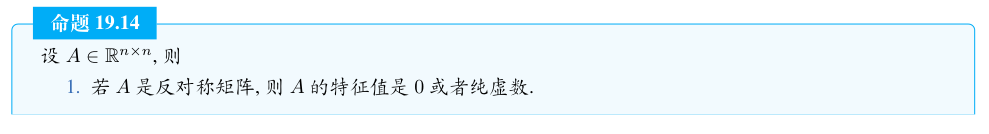
\includegraphics[width=\textwidth]{6-cmc决赛-2025040618.png}
% \caption{}
\label{}
\end{figure}
\begin{figure}[H]
\centering
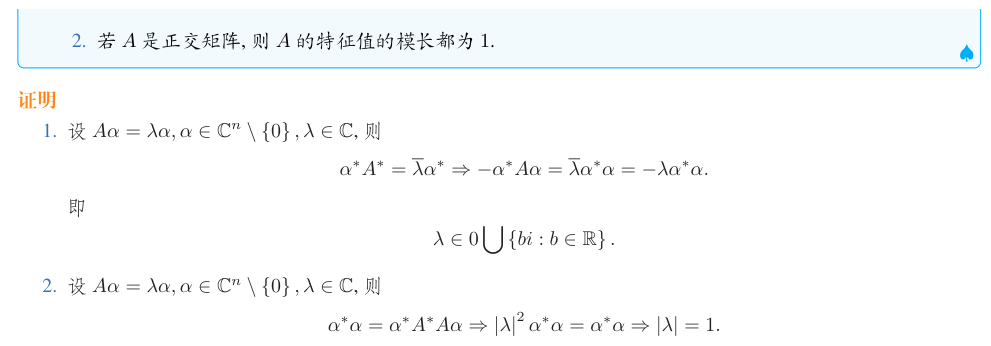
\includegraphics[width=\textwidth]{7-cmc决赛-2025040618.png}
% \caption{}
\label{}
\end{figure}
\begin{figure}[H]
\centering
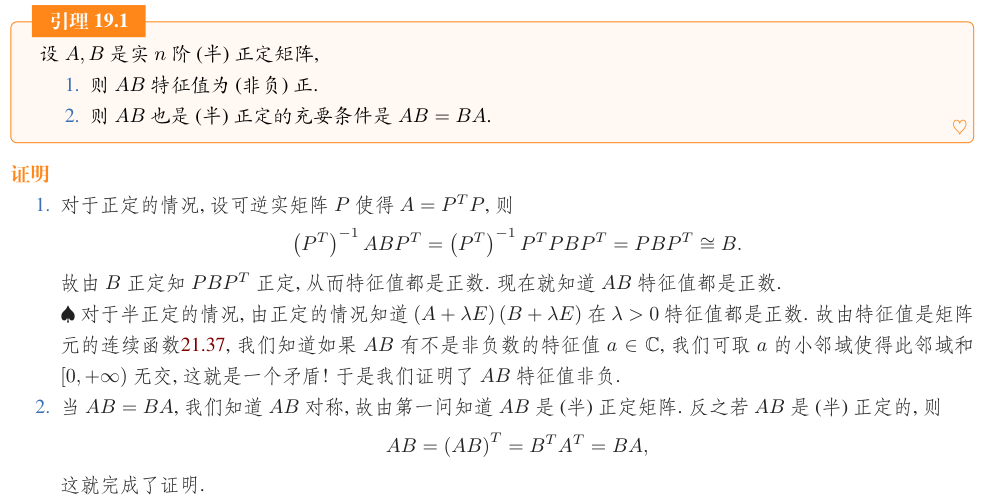
\includegraphics[width=\textwidth]{8-cmc决赛-2025040618.png}
% \caption{}
\label{}
\end{figure}
\begin{figure}[H]
\centering
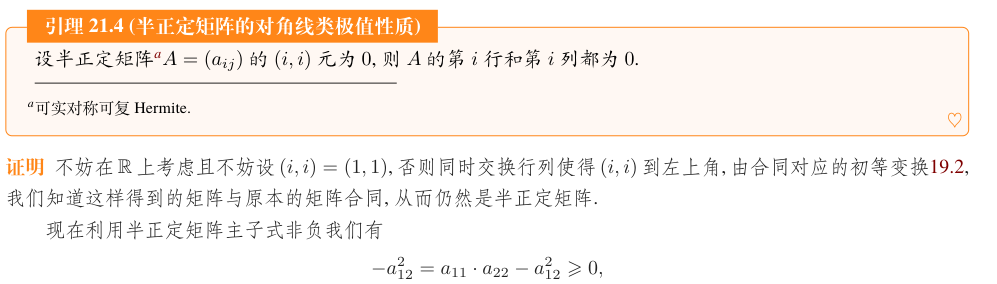
\includegraphics[width=\textwidth]{9-cmc决赛-2025040618.png}
% \caption{}
\label{}
\end{figure}
\begin{figure}[H]
\centering
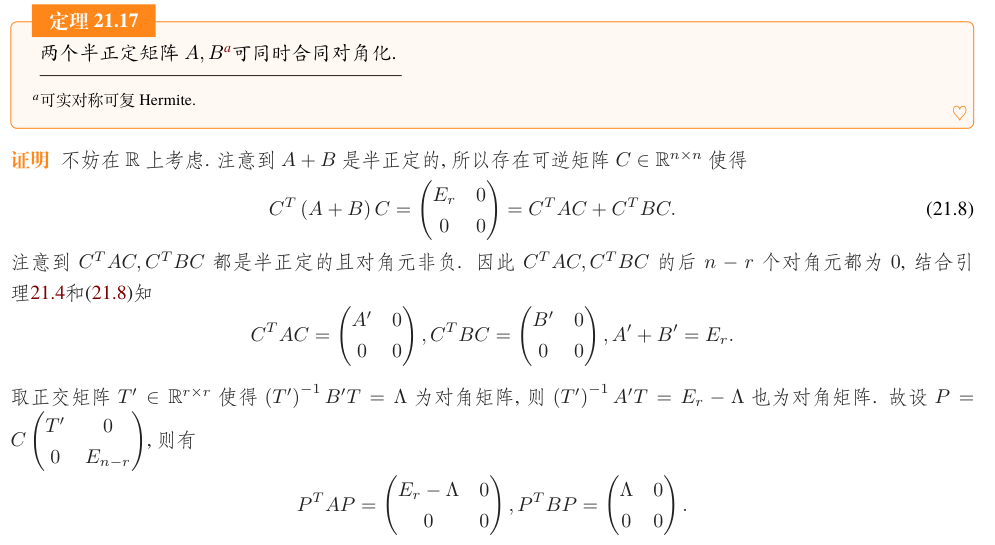
\includegraphics[width=\textwidth]{10-cmc决赛-2025040618.png}
% \caption{}
\label{}
\end{figure}
\begin{figure}[H]
\centering
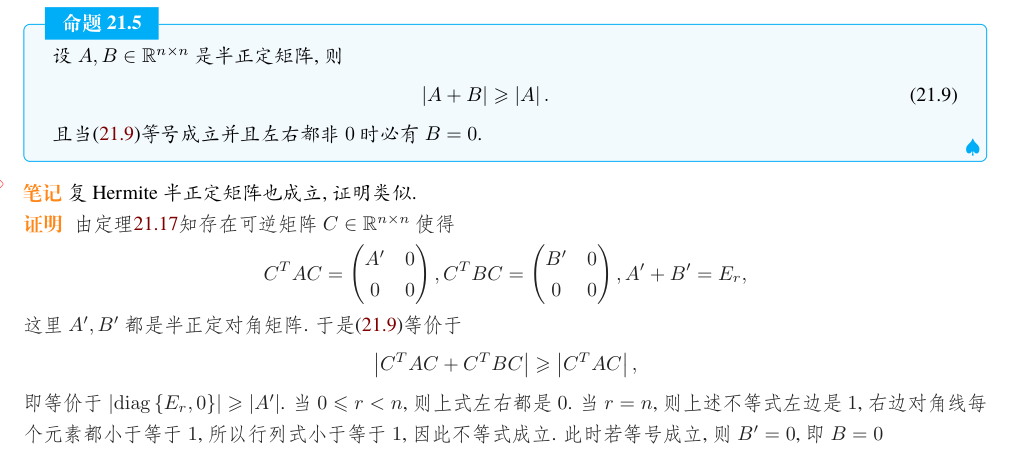
\includegraphics[width=\textwidth]{11-cmc决赛-2025040618.png}
% \caption{}
\label{}
\end{figure}
\begin{figure}[H]
\centering
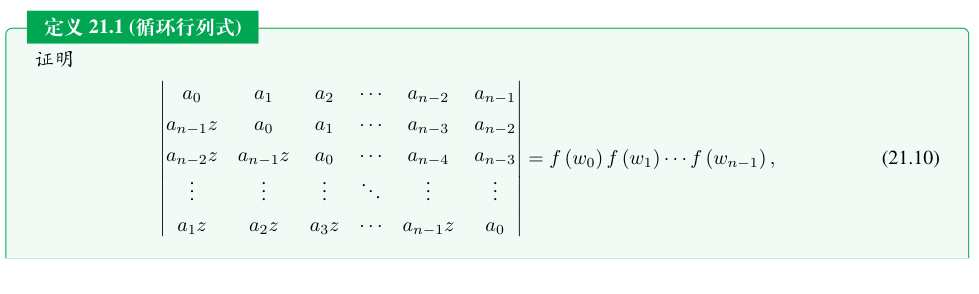
\includegraphics[width=\textwidth]{12-cmc决赛-2025040618.png}
% \caption{}
\label{}
\end{figure}
\begin{figure}[H]
\centering
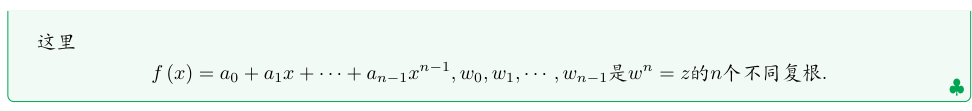
\includegraphics[width=\textwidth]{13-cmc决赛-2025040618.png}
% \caption{}
\label{}
\end{figure}
\begin{figure}[H]
\centering
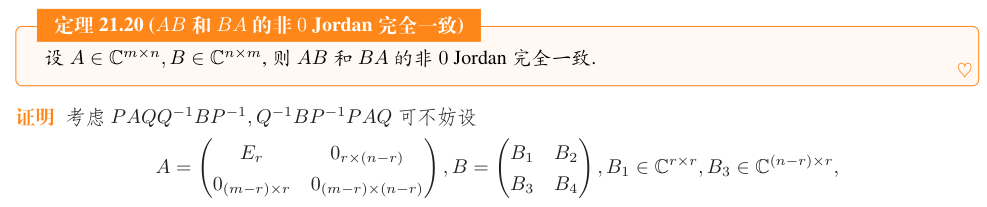
\includegraphics[width=\textwidth]{14-cmc决赛-2025040618.png}
% \caption{}
\label{}
\end{figure}
\begin{figure}[H]
\centering
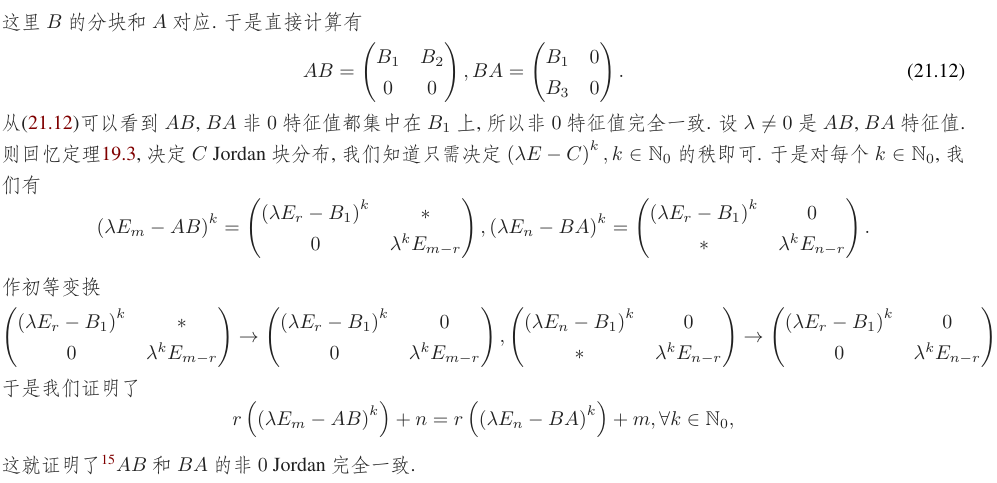
\includegraphics[width=\textwidth]{15-cmc决赛-2025040618.png}
% \caption{}
\label{}
\end{figure}

\begin{figure}[H]
\centering
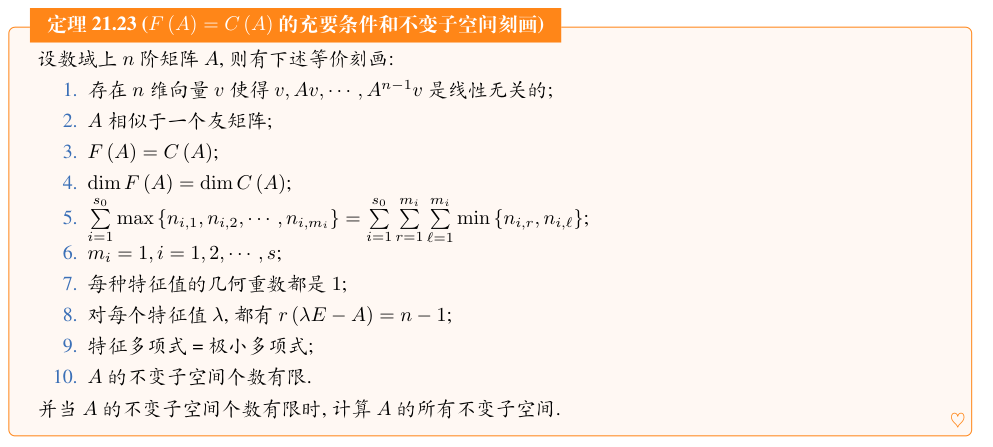
\includegraphics[width=\textwidth]{16-cmc决赛-2025040618.png}
% \caption{}
\label{}
\end{figure}
\begin{figure}[H]
\centering
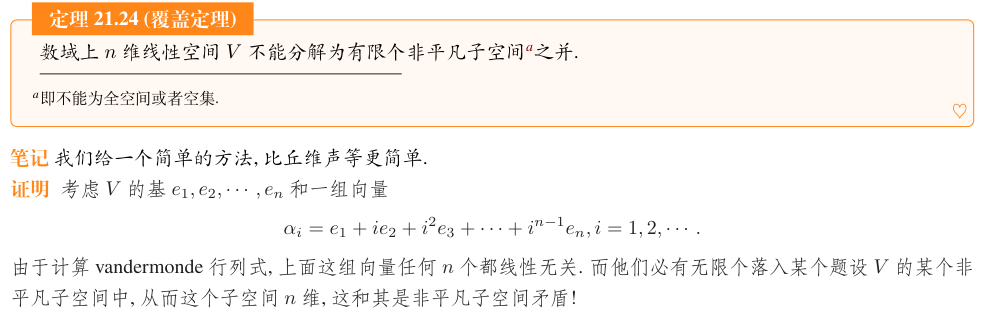
\includegraphics[width=\textwidth]{17-cmc决赛-2025040618.png}
% \caption{}
\label{}
\end{figure}
\begin{figure}[H]
\centering
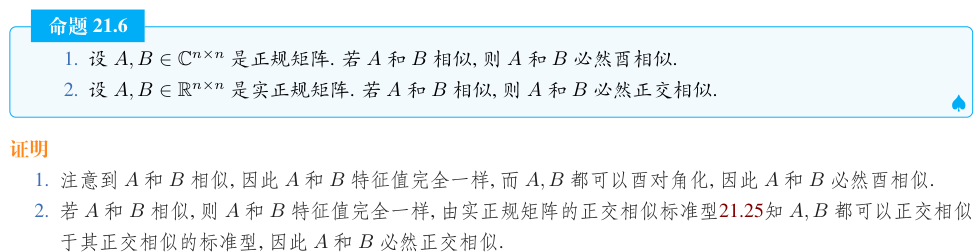
\includegraphics[width=\textwidth]{18-cmc决赛-2025040618.png}
% \caption{}
\label{}
\end{figure}
